\chapter*{درباره‌ی نویسنده}
\addcontentsline{toc}{chapter}{درباره‌ی نویسنده}
\markboth{درباره‌ی نویسنده}{درباره‌ی نویسنده}

\noindent
\begin{LR}
\begin{minipage}[t]{0.34\textwidth}
    \centering
    \vspace{0pt}
    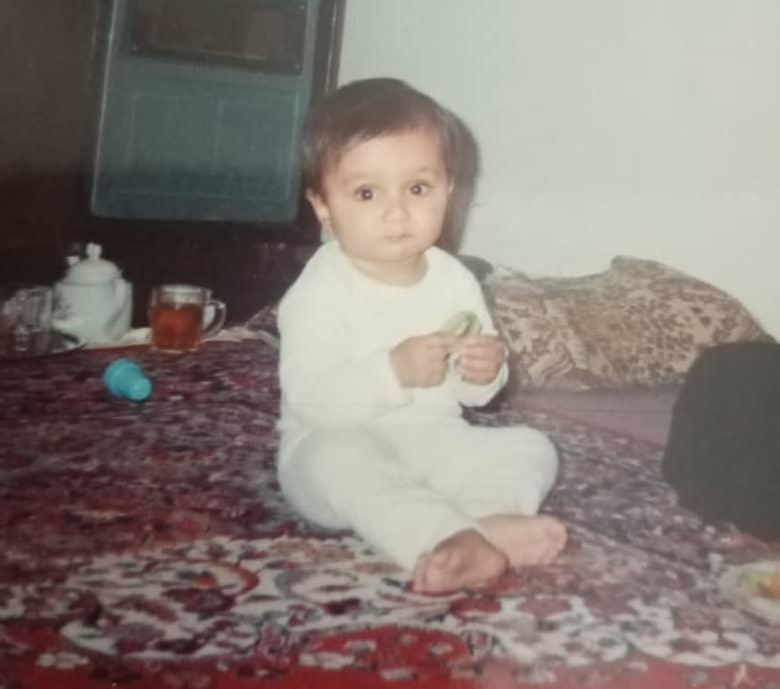
\includegraphics[width=\linewidth]{../../shared/images/author-photo.jpg}
\end{minipage}
\hfill
\begin{minipage}[t]{0.62\textwidth}
    \begin{RTL}
    \small
    \setlength{\parskip}{0.45em}
    \setlength{\parindent}{0pt}

    \textbf{\BookletAuthor} (\lr{\BookletAuthorHandle}) دانشجوی
    مهندسی کامپیوتر و برنامه‌نویس متن‌باز است که علاقه‌اش به
    کامپیوتر از حدود چهارسالگی شروع شده، وقتی کامپیوتر بیشتر
    ابزاری برای بازی و کنجکاوی بود. در سیزده یا چهارده‌سالگی، مدت‌ها
    پیش از آنکه اولین خط کد را بنویسد، اولین کتابش را نوشت: یک
    داستان کوتاه و تخیلی درباره‌ی دایناسورها.

    همان کنجکاوی بعدها به توسعه‌ی بک‌اند و ساختن چند ابزار متن‌باز
    رسید. پرسشی ساده، \emph{«آرایه چیست؟»}، او را از مرزهای
    برنامه‌نویسی مقدماتی گذراند و به لایه‌بندی حافظه و معماری
    پردازنده رساند. \textit{آرلیز} حاصل مکتوب همین جست‌وجوست، و
    این کتابچه یک تکه‌ی کوچک از آن است.
    \end{RTL}
\end{minipage}
\end{LR}

\medskip

\noindent
\begin{RTL}
\begin{tabular}{@{}ll}
ایمیل: & \href{mailto:\BookletEmail}{\lr{\BookletEmail}} \\
هندل: & \lr{\BookletAuthorHandle} \\
مخزن: & \href{https://github.com/papyrxis/arliz}
         {\lr{github.com/papyrxis/arliz}} \\
\end{tabular}
\end{RTL}

\clearpage